\documentclass[12pt]{article}
\usepackage[utf8]{inputenc}

\usepackage[margin=3cm]{geometry}
\setlength{\parindent}{0pt}

\usepackage{amsmath}
\usepackage{amssymb}
\usepackage{amsthm}

\usepackage[usenames,dvipsnames]{xcolor}
\usepackage{graphicx}
\usepackage{wrapfig}
\usepackage{float}
\usepackage{caption}
\usepackage{subcaption}
\graphicspath{ {figures/} }

\newcommand \dir[1] {\textbf{\textit{#1}}}
\newcommand \tabbox[1] {\underline{#1}}
\newcommand \elem[1] {{\color{red} #1}}

\begin{document}

\title{ Interface manual }
\maketitle

\section{Introduction}

\begin{wrapfigure}{r}{0.45\textwidth}
	\begin{subfigure}{0.5\textwidth}
		\centering
		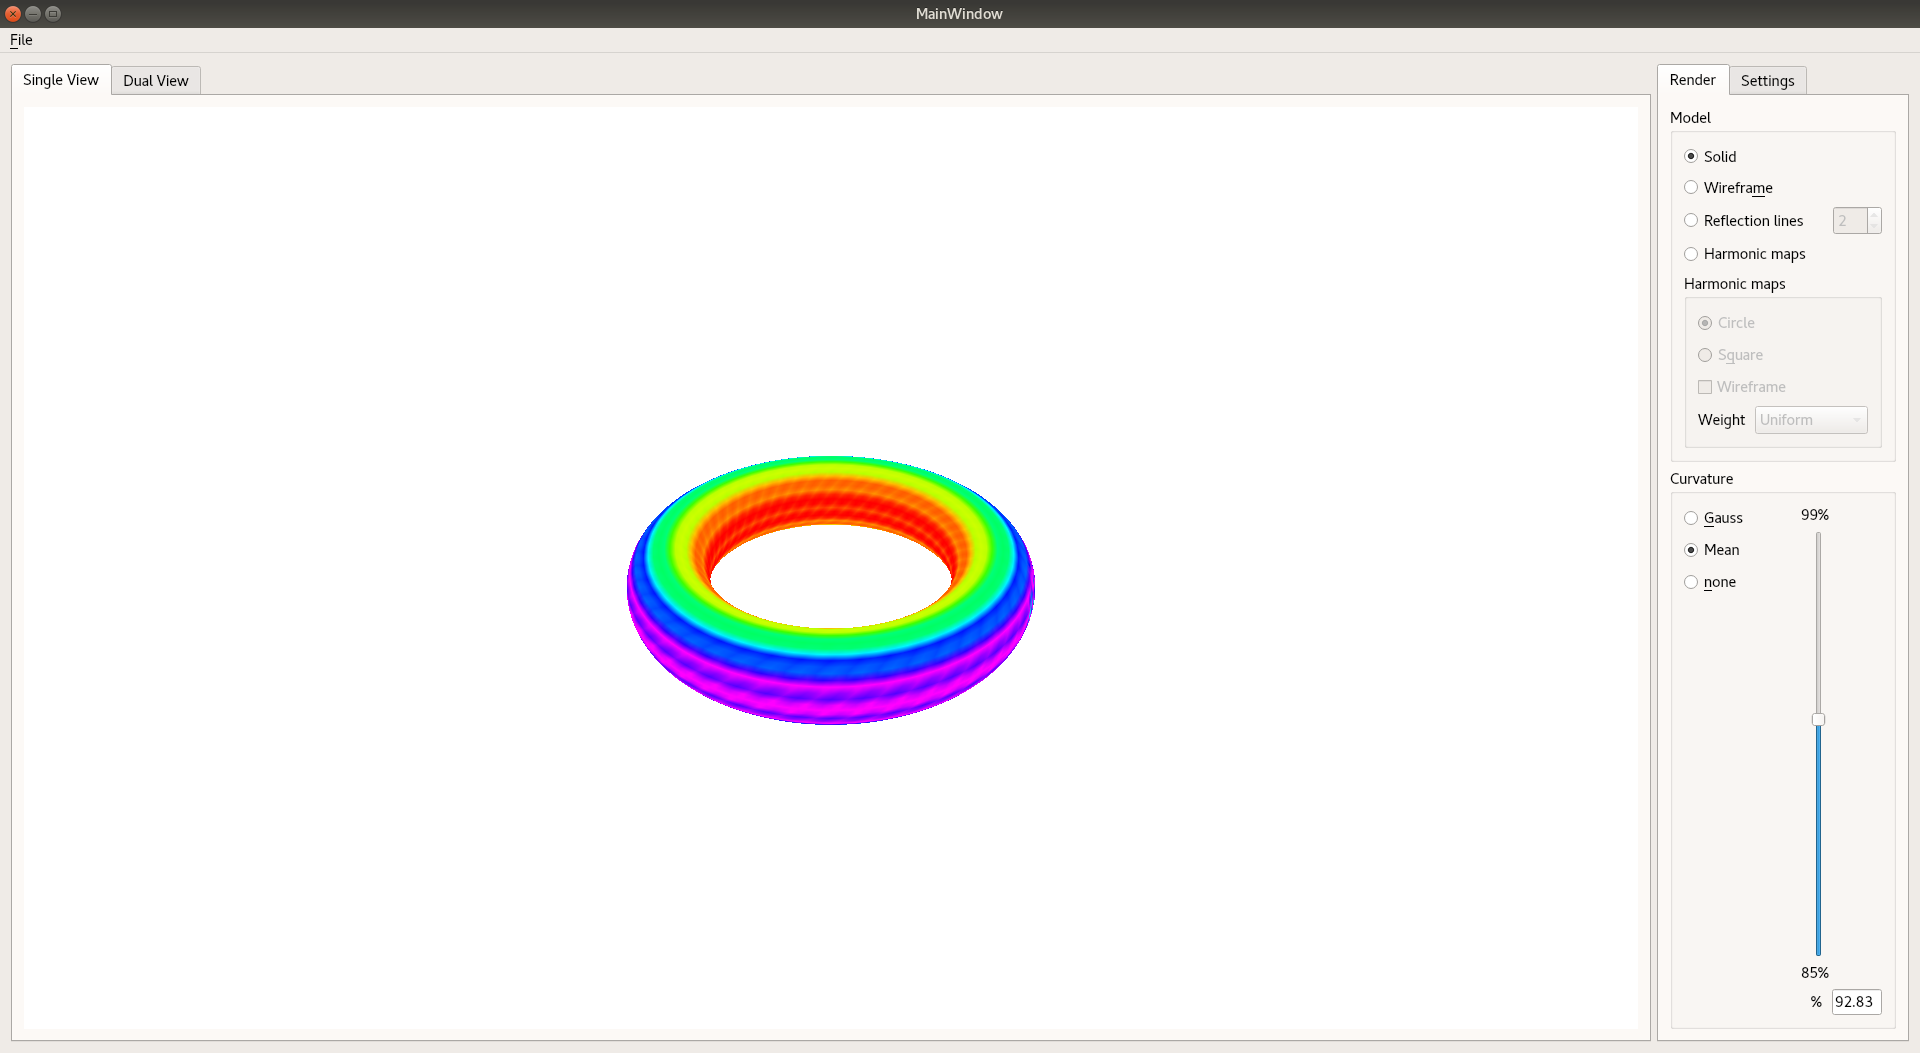
\includegraphics[scale=0.1]{single-view}
		\caption{Single view.}
	\end{subfigure}
	\begin{subfigure}{0.5\textwidth}
		\centering
		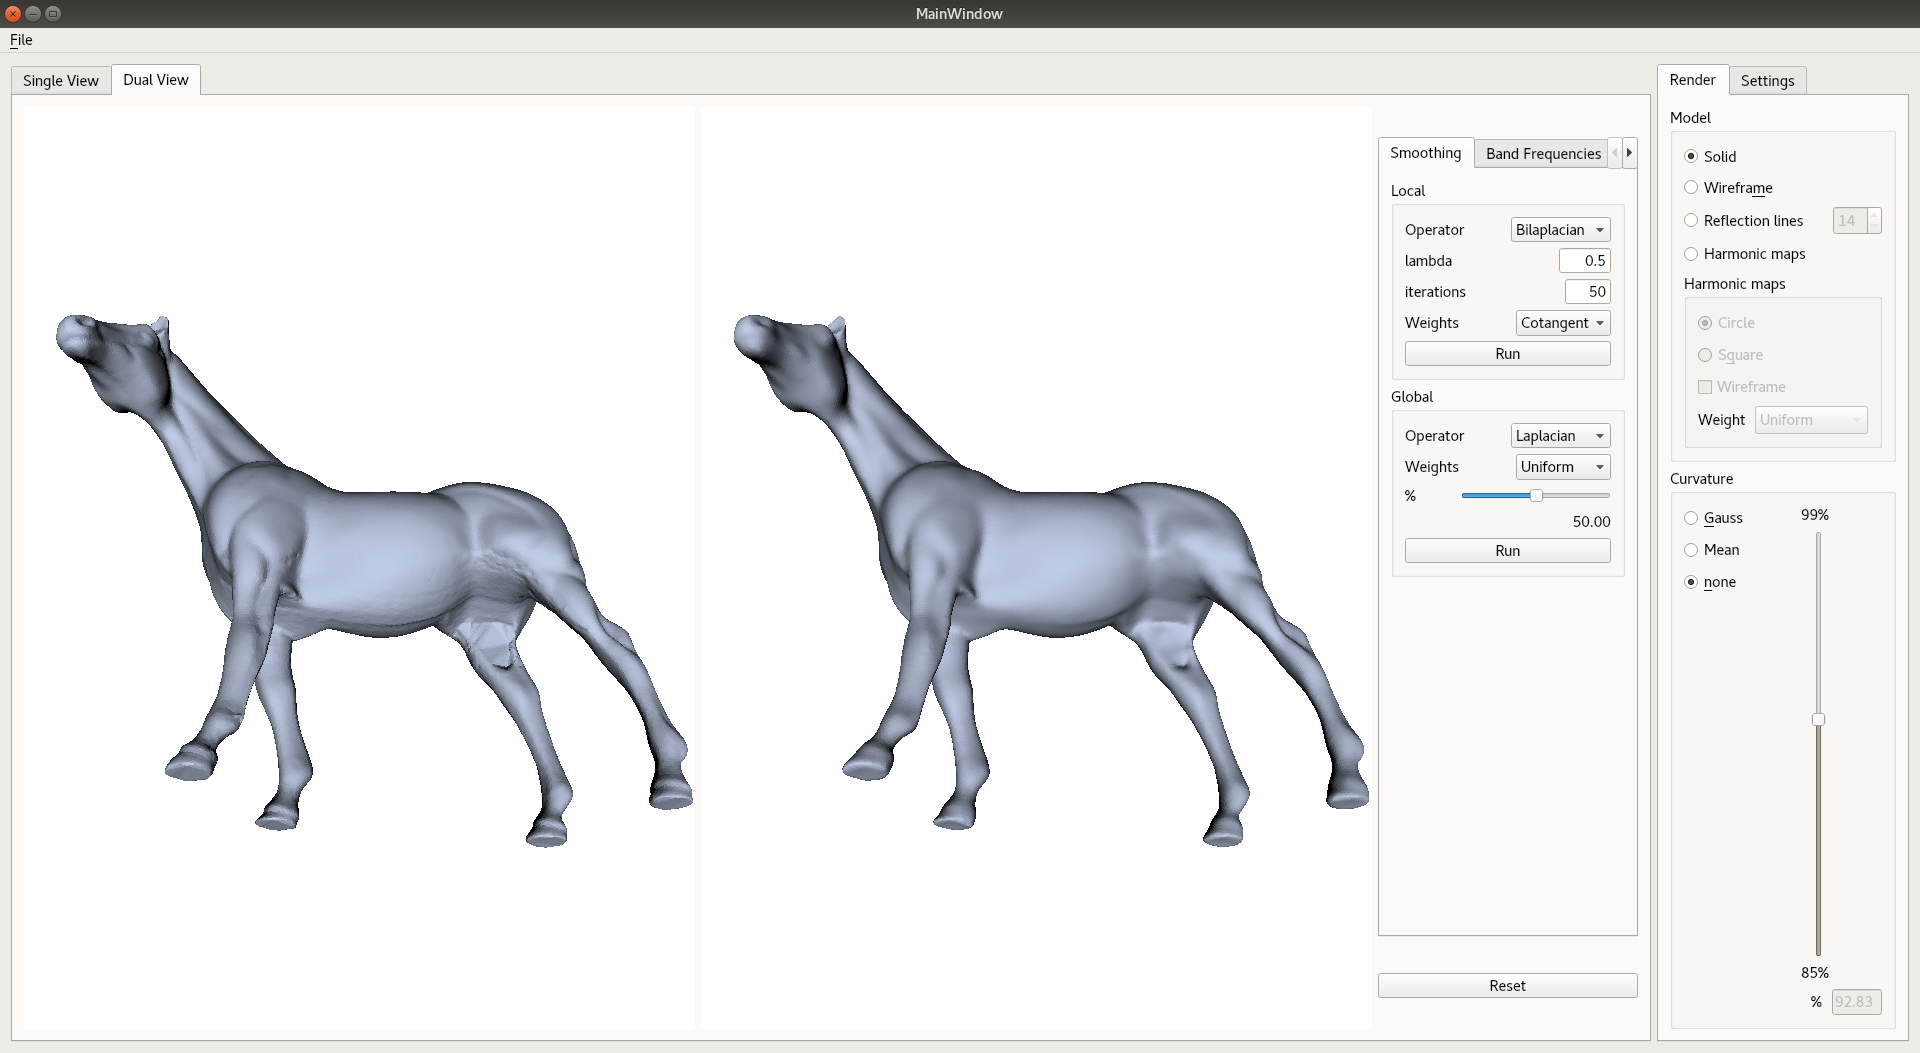
\includegraphics[scale=0.1]{dual-view}
		\caption{Dual view.}
	\end{subfigure}
	\vspace{-10pt}
\end{wrapfigure}

The interface is divided into two views: single view and dual view.
\begin{itemize}
	\item Single view contains two tabs: rendering and settings.
	These two are still accessible in the dual view. The operations
	they offer are explained in section \ref{sec:single-view}.
	
	\item Dual view contains three tabs, and its main characteristic
	is that it provides two viewers. Both viewers start with the same
	mesh and only the mesh in the right viewer is modified. This is
	useful for comparing the result of applying the operations accessible
	through the 3 different tabs in this view. These operations are
	explained in section \ref{sec:dual-view}.
\end{itemize}

All viewers (in both the single and dual view) allow the user to rotate
the mesh and zoom in and out.

\hfill

The full project (code and documentation) can be found via this link:
\begin{verbatim}
https://github.com/lluisalemanypuig/geometry-processing/
\end{verbatim}
The full details on what each option does can be found in the doxygen
documentation of the library, in the directory \dir{geoproc-docs}.
The code of the library can be found in the directory \dir{geoproc},
and a command-line application to apply the algorithms implemented can
be found in the directory \dir{command-line}. The code of the
interface can be found in the directory \dir{interface}.

\hfill

See section \ref{sec:functionalities} to see the state of functionality
of every algorithm (what works at a 100\%, what is not implemented, ...).
See the project's \textbf{README.md} file for instructions on how to
compile the project.

\section{Single View}
\label{sec:single-view}

The operations accessible in this view are divided into two tabs.
The most simple one is the \tabbox{Settings} tab. This contains the
option to increase the number of threads that the algorithms can use
to speed-up the software (see section \ref{sec:parallel-algorithms}
to see what features benefit from increasing the number of threads).
There is also the option to clean up the loaded meshes.

\hfill

\begin{wrapfigure}{r}{0.3\textwidth}
	\vspace{-30pt}
	\begin{subfigure}{0.4\textwidth}
		\centering
		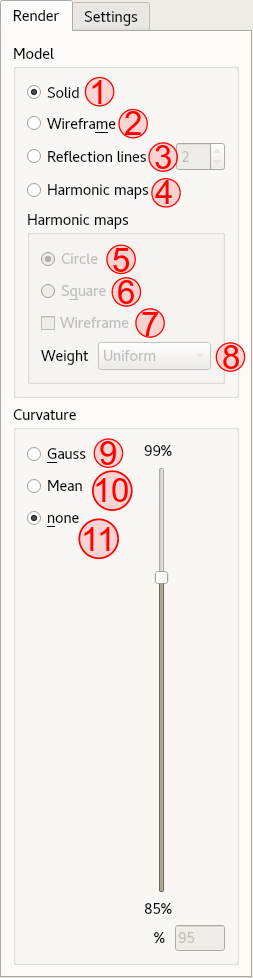
\includegraphics[scale=0.175]{SV-render}
		\caption{Render tab.}
	\end{subfigure}
	\begin{subfigure}{0.4\textwidth}
		\centering
		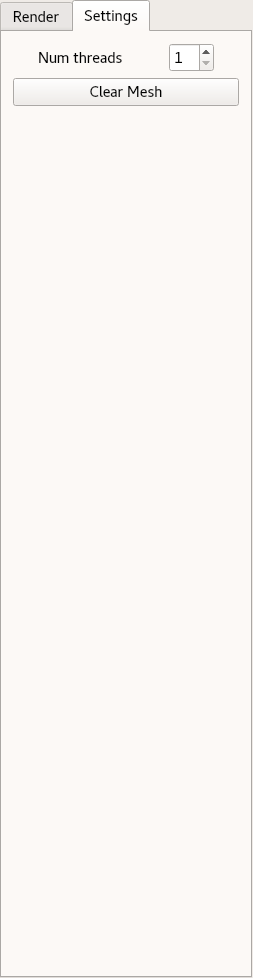
\includegraphics[scale=0.8]{SV-settings}
		\caption{Settings tab.}
	\end{subfigure}
	\caption{Tabs of single view.}
	\vspace{-30pt}
\end{wrapfigure}

The operations in the \tabbox{Render} tab are meant to only change the
way a mesh is rendered. One can visaulise the Gaussian and Mean curvature
of a mesh, in the \tabbox{Curvature} box. Since the curvature values
can range from a really small value to a really high one, most of the
values being clustered to one end of the spectrum, a slider has been
provided to let the user choose how many of these curvature values should
be taken into account when coloring the vertices of the mesh using them.

\hfill

Also, the renderisation of the mesh can be modified in the \tabbox{Model}
box:
\begin{itemize}
	\item We can render it either in solid mode (\elem{1}), or wireframe
	(\elem{2}).
	\item Reflection lines (\elem{3}) on the loaded mehs can be visualised.
	The amount of reflection lines to consider can be modified.
	\item We can render the mesh
	with a procedurally generated texture on it using the Harmonic Maps
	parametrisation (\elem{4}). This parametrisation can only be done in
	meshes with a single boundary. This parametrisation starts distributing
	the vertices on this boundary on either a circle (\elem{5}) or on a
	square (\elem{6}). Computing the coordinates of the texture can be
	done either using Uniform or Cotangent weights (\elem{8}). Finally,
	this parametrisation can be rendered to look like a remeshing (\elem{7}).
\end{itemize}

\section{Dual View}
\label{sec:dual-view}

Dual view offers several operations. As mentioned in the introduction,
this view is split into two viewers and these operations only affect the
mesh in the right viewer. The tabs, to the right of the viewers and to the
left of the operations available for both views, classify the operations
into three categories:
\begin{itemize}
	\item \tabbox{Smoothing} (see section \ref{sec:dual-view:smoothing}).
	\item \tabbox{Band frequencies} (see section \ref{sec:dual-view:band-frequencies}).
	\item \tabbox{Remesing} (see section \ref{sec:dual-view:remeshing}).
\end{itemize}

One common option to all these categories is to reset the mesh in the
right viewer: it takes the unmodified mesh in the left viewer and sets
it to the one to the right. In order to have these operations applied,
the user has to click on the corresponding \textit{Run} button.

\begin{figure}[H]
	\centering
	\begin{subfigure}{0.32\textwidth}
		\centering
		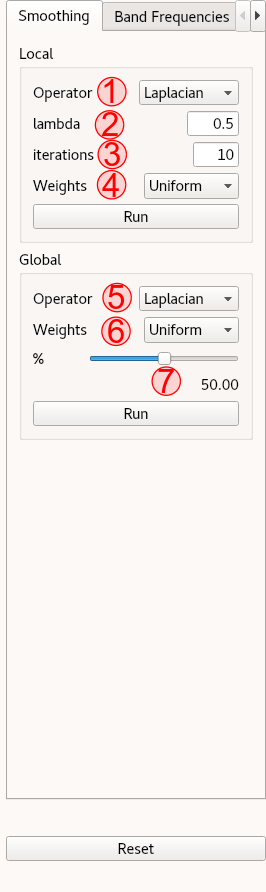
\includegraphics[scale=0.24]{DV-smoothing}
		\caption{Smoothing.}
		\label{fig:DV:smoothing}
	\end{subfigure}
	\begin{subfigure}{0.32\textwidth}
		\centering
		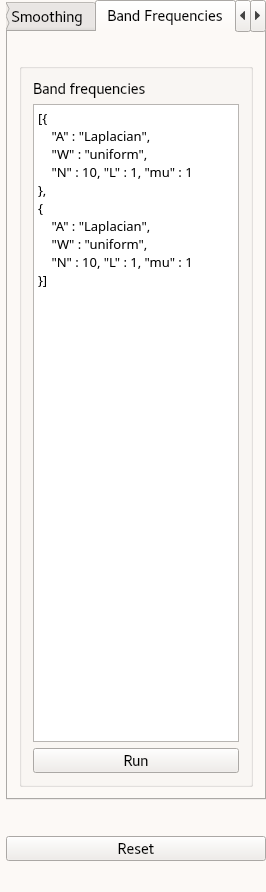
\includegraphics[scale=1]{DV-band-frequencies}
		\caption{Band frequencies.}
		\label{fig:DV:band-freqs}
	\end{subfigure}
	\begin{subfigure}{0.32\textwidth}
		\centering
		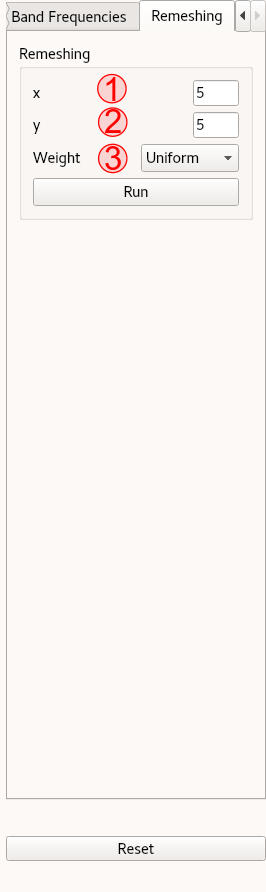
\includegraphics[scale=0.24]{DV-remeshing}
		\caption{Remeshing.}
		\label{fig:DV:remeshing}
	\end{subfigure}
	\caption{Tabs of dual view.}
\end{figure}

\subsection{Smoothing}
\label{sec:dual-view:smoothing}

In this tab the user has access to two categories of smoothing algorithms:
local and global (see figure \ref{fig:DV:smoothing}).

\subsubsection{Local}
Here the user can choose between three operators: Laplacian, BiLaplacian,
Taubin-$\lambda\mu$ (\elem{1}). The value of the $\lambda$ coefficient
can be set by the user (\elem{2}), also the amount of iterations (\elem{3})
that the local algorithm should perform, and the type of weight: Uniform or Cotangent
(\elem{4}).

\subsubsection{Global}
The global smoothing algorithm is only implemented for the Laplacian
opearator (\elem{5}). The user, however, is able to choose the type of
weight: Uniform or Cotangent (\elem{6}). Additionally, the user can
select the amount of fixed vertices that the algorithm needs to perform
the smoothing. This amount is given using the slider that specifies the
percentage of vertices to be fixed (\elem{7}).

\subsection{Band frequencies}
\label{sec:dual-view:band-frequencies}

This tab allows the user to apply several smoothing options to the mesh
in the right viewer (see figure \ref{fig:DV:band-freqs}). These operations
have to be described by writing a list of JSON-formatted operations.

\hfill

Formally, the operations applied to the mesh are:
\[
M' = M + \sum_{i=1}^n \mu_i \cdot D_i
\]
where the band frequencies $D_i$ are defined as:
\[
D_i = S_i(M) - S_{i + 1}(M)
\]
In these expressions, $M$ and $M'$ denote the input and output meshes,
respectively. The coefficient $\mu_i$ is the weight of each band frequency
and $S_i(M)$ is the result of applying a smoothing algorithm on the input
mesh $M$.

\subsubsection{Format of the text}

The description of the operations is a JSON list of at least two band
frequencies. Each band frequency is defined using a brace-enclosed list
of options. In the following example we can see the options that need to
be given:
\begin{verbatim}
{
    "A" : "Laplacian",                  1
    "W" : "Uniform",                    2
    "N" : 10,                           3
    "L" : 1,                            4
    "mu" : 1                            5
}
\end{verbatim}
\begin{enumerate}
	\item Specify smoothing operator. Must be a string.
	\hfill
	
	Allowed values: Laplacian, BiLaplacian, TaubinLM.
	\item Specify type of weight. Must be a string.
	\hfill
	
	Allowed values: Uniform, Cotangent.
	\item Specify a number of iterations. Must be an integer.
	\item Specify value of $\lambda$, the coefficient for the smoothing
	algorithm. Must be a floating-point value.
	\item Specify value of $\mu$, the weight of this band frequency.
	Must be a floating-point value. Although it will be ignored, the last
	band frequency can also have this option.
\end{enumerate}

Needles to say that the numbers to the right-most part of the example
should not be included in the interface.

\subsection{Remeshing}
\label{sec:dual-view:remeshing}

See figure \ref{fig:DV:remeshing} for a screenshot of this tab.
Remeshing does two things. First, it computes the Harmonic Maps parametrisation
of the input mesh \textbf{using the ``Square'' shape} (see bullet list of
section \ref{sec:single-view}). Then, applies the remeshing. This remeshing is
guided by the amount of points the regular grid will have in the $x$- and
$y$- axis (\elem{1} and \elem{2} respectively), and the weight type (\elem{3}).

\section{Parallelised algorithms}
\label{sec:parallel-algorithms}

Here are listed the options that can take advantage of the use of
several threads:
\begin{itemize}
	\item The computation of the curvature values. Their visualtion, however,
	does not use multithreading.
	\item All the local smoothing algorithms (that is, for all the operators
	available).
	\item Since band frequencies use local smoothing algorithms, this
	option can benefit from using multithreading too.
	\item Part of the remeshing algorithm has been parallelised. Since
	the parametrisation using Harmonic Maps is not parallel, only the
	construction of the new mesh is actually parallel.
\end{itemize}

\section{Status of functionalities}
\label{sec:functionalities}

All features provided in the interface are fully functional, except for
the following:
\begin{itemize}
	\item Reflection lines rendering mode. Reflection lines are perfectly
	rendered for those models in which the normals needed for this purpose
	(see next paragraph) can be computed as the normal of every triangle
	(if a triangle has vertices $v_i$, $v_j$ and $v_k$ then its normal is
	the normalisation of $(v_j - v_i) \times (v_k - v_i)$). A model of a
	completely flat surface, for example, is perfectly suitable for this
	rendering mode.
	\hfill
	
	Ideally, the normals to be used in order to render these lines
	properly should be computed differently (not done). The normals of all
	triangles should be computed as the average of \textbf{some} of their
	neighbouring faces. In this project, the normals are taken as the cross
	product, as explained before.
	
	\item Global smoothing. Only the Laplacian operator is implemented
	for this algorithm.
	
	\item Remeshing. Remeshing is not implemented for the shape ``circle''.
\end{itemize}

\end{document}
